\section{Introduction}
\label{sec:intro}

An engineering agent can be excellent at choosing among feasible candidates and still be poor at finding one. In DiagBench, model_B is the strongest constrained-repair model in P2 (0.390 final feasible power ratio) but only seventh on P4 full-order ranking (0.824 Kendall Tau). model_C shows the opposite profile: it leads P4 (0.887 Tau) but is near the bottom on P2 (0.133 ratio). If engineering competence were a scalar, such reversals should be rare. They are instead one of the most stable patterns we observe. This suggests that engineering-agent readiness is best diagnosed not by one aggregate capability score, but by whether a model's default behavioral style matches the demands of each engineering decision.

Existing benchmarks leave this mismatch hard to see. SWE-bench~\citep{jimenez2024swebench}, LiveCodeBench~\citep{jain2024livecodebench}, MLE-bench~\citep{chan2025mlebench}, AgentBench~\citep{liu2024agentbench}, and related suites evaluate realistic agent workflows, but endpoint pass/fail usually does not identify which internal engineering decision failed. Multi-agent frameworks such as AutoGen~\citep{wu2023autogen} and MetaGPT~\citep{hong2024metagpt} show that language agents can coordinate through conversation, but in physical design language-only closure can amplify wrong physical intuitions rather than falsify them. Classical optimization suites such as COCO/BBOB~\citep{hansen2021coco} measure search under objective feedback, but they do not test whether an agent should enter search, recover from a corrupted trajectory, or choose among feasible designs under an explicit engineering policy.

We therefore frame engineering-agent evaluation around two concepts. A \textbf{response-control prior} is a model's default behavioral style before any explicit reasoning fully unfolds: action discipline, edit style, feedback obedience, state trust, and preference execution. A \textbf{trusted-state boundary} is a workflow checkpoint where the valid state representation, allowed action, and failure consequence change. The central thesis of this paper is that model performance is usefully diagnosed through prior-boundary compatibility: observed strengths and failures are strongly associated with how a model's default behavior aligns with the specific boundary it is asked to cross. We ask four questions: do frontier models dissociate across trusted-state boundaries (RQ1); is corrupted-state recovery distinct from clean-start repair (RQ2); is feasible-set selection distinct from feasible-set construction (RQ3); and can response-control profiles be quantified from existing logs (RQ4)?

\begin{figure*}[t]
\centering
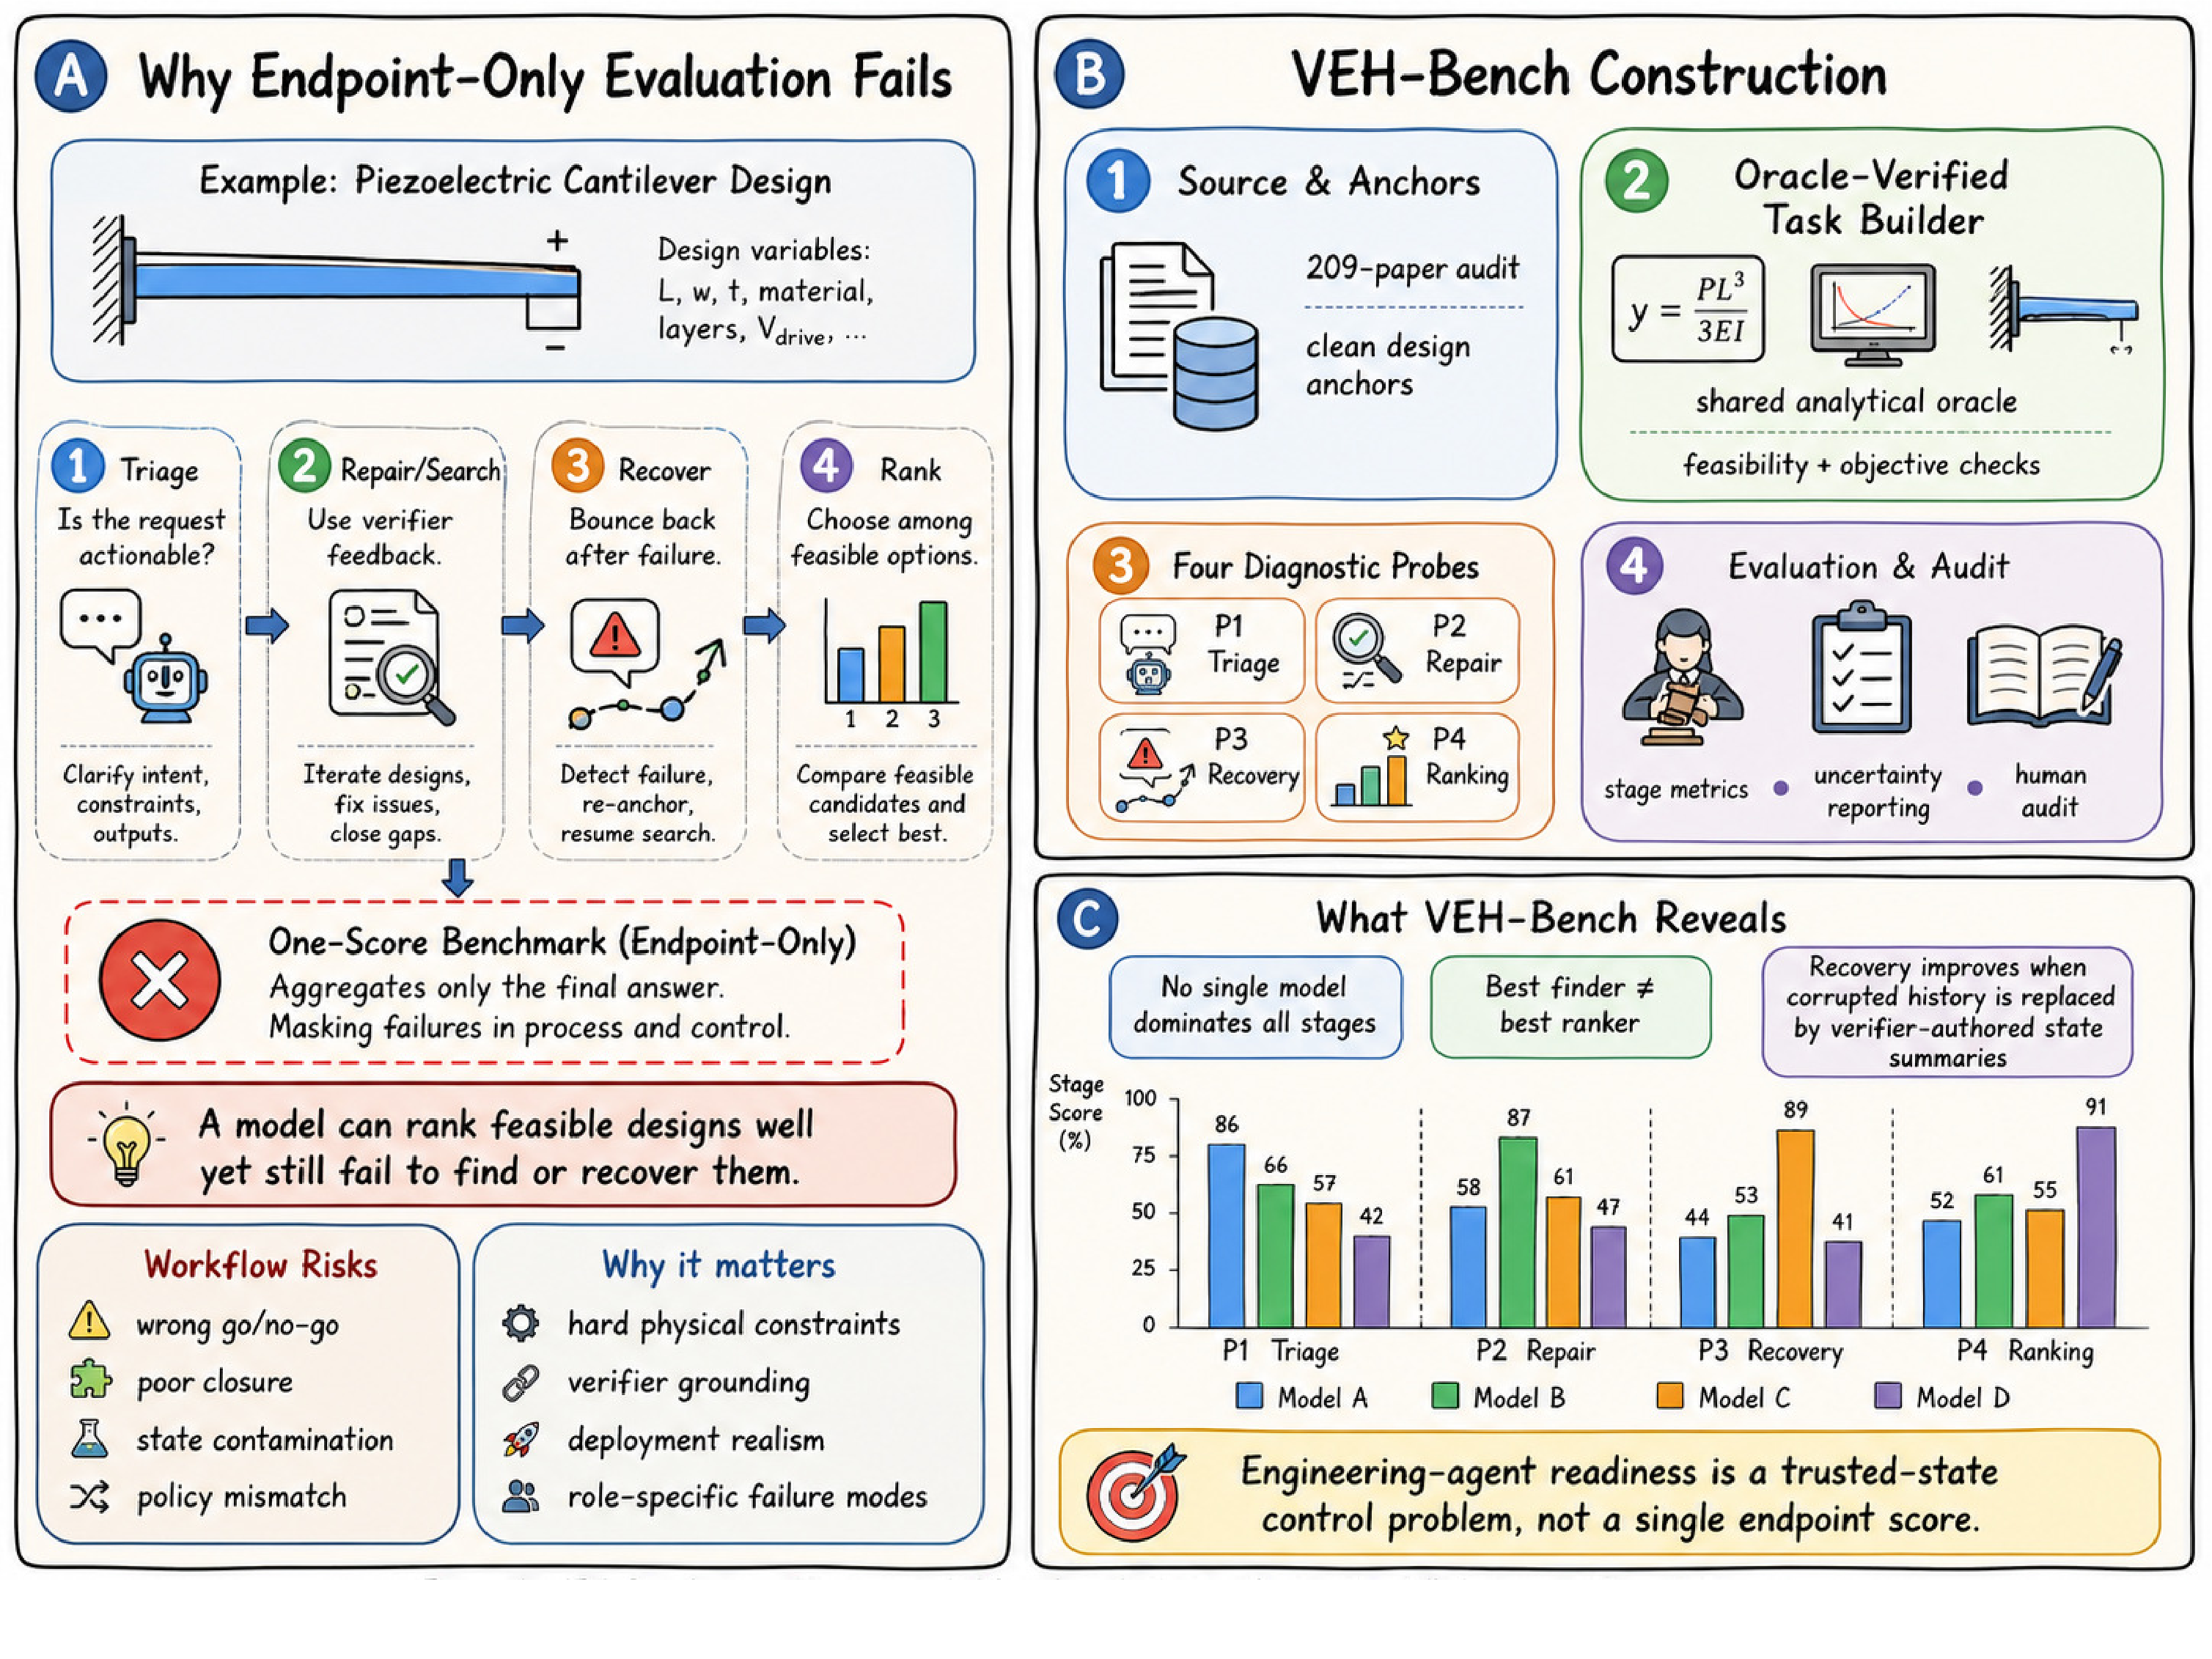
\includegraphics[width=\linewidth]{figures/main/running_example.pdf}
\caption{DiagBench overview. Endpoint-only evaluation masks where engineering agents fail; VEH-Bench turns source-grounded anchors into oracle-verified P1--P4 probes and reports stage-local failures rather than a single endpoint score.}
\label{fig:running_example}
\end{figure*}

Three design challenges follow. First, physical validity must be externally adjudicated: once feasibility is negotiated only inside language, a wrong trajectory can become contaminated evidence. Second, the benchmark must decompose the workflow rather than merely make one long task harder, because a harder repair task still does not test triage, recovery, or policy-conditioned selection. Third, the benchmark must show that non-monotonic rankings are structural rather than noise; otherwise stage decomposition would be redundant.

DiagBench addresses these challenges with a verifier-grounded benchmark for engineering design agents. The current VEH instantiation contains 763 manifest-backed tasks derived from a 209-paper extraction audit, 52 cleaned structure-review anchors, DOI-disjoint optimizer-facing splits for P2--P4, and a shared analytical oracle. The four probes correspond to four trusted-state boundaries: P1 tests credible triage before search, P2 tests constrained repair under verifier feedback, P3 tests recovery after a corrupted trajectory, and P4 tests policy-conditioned ranking among feasible candidates. Figure~\ref{fig:running_example} gives the motivation and benchmark overview; Figure~\ref{fig:workflow} summarizes the full workflow design.

Our contributions are:
\begin{itemize}[leftmargin=5mm,itemsep=1mm,topsep=1mm]
    \item We propose a workflow-structured evaluation framework that separates four trusted-state boundaries and interprets stage dissociation through response-control prior-boundary mismatch (Sections~\ref{sec:method} and~\ref{sec:experiments}).
    \item We instantiate the framework as a 763-task VEH benchmark with manifest-backed provenance, a shared analytical oracle, and a documented construction path from extraction audit to released task banks (Section~\ref{sec:method}; Appendix).
    \item Across 12 complete model runs with explicit run-mode tags, we show that no model dominates all four stages; log-derived profile indicators strongly track stage outcomes, including action prior to P1 ($\rho=0.97$), edit style to P2 ($\rho=0.84$), and preference execution to P4 ($\rho=0.77$) (Section~\ref{sec:experiments}).
    \item We provide mechanism evidence: a 36-task P3 state-summary intervention improves recovery by 13.2 points and cuts cascade by 18.6 points, while a matched isomorphic probe shows a 26--61 point gap between feasible-set selection and construction (Section~\ref{sec:experiments}).
    \item We add a hardened closed-form circuit audit showing that the P1--P4 diagnostic framework transfers to a second engineering domain, while model rankings remain boundary-specific rather than globally monotonic (Section~\ref{sec:experiments}; Appendix).
\end{itemize}
